\subsection{Kommunikation}\label{subsec: Kommunikation} \todo{anpassen}
\subsubsection{WLAN Konfiguration}\label{subsub: Wlan Konfiguration}
Die Funkkommunikation zwischen Sensor, Aktor und MQTT-Brocker wird mittels Wireless Local Area Network (WLAN) auf dem OSI layer 1 stattfinden. Um die einzelnen Target also Sensoren und Aktoren in das Lokale Netzwerk zu verbinden, wird beim Starten des ESP32 ein Accespoint eröffnet. Für diesen WiFi-Manager Prozess wird eine Bibliothek eingebunden. Die benötigte Bibliothek steht auf Github zur Verfügung \cite{zhouhan0126_zhouhan0126/wifimanager-esp32_2019}. 

\begin{figure}[H]
	\centering
	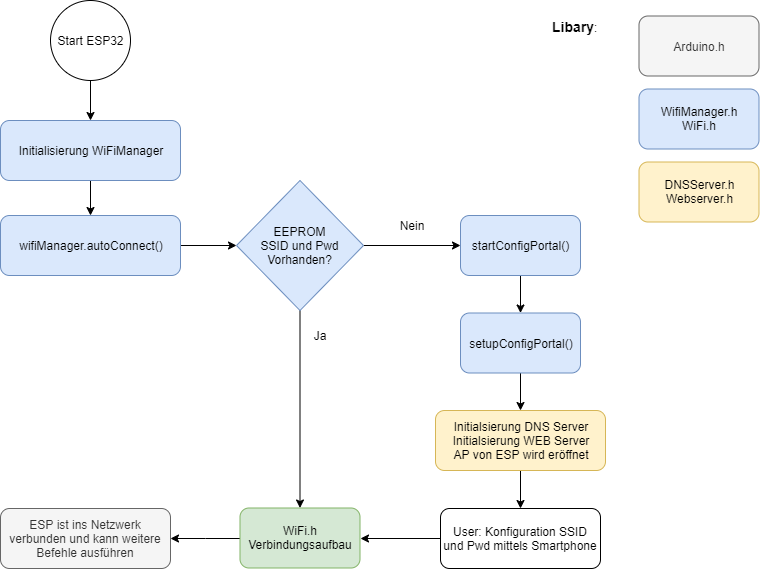
\includegraphics[width=\textwidth]{graphics/statediagramWiFi.png}
	\caption{Statediagram Verbindungsaufbau ESP ins Netzwerk mit einem AP}
	\label{pic: statediagramWiFi}
\end{figure}   

Wird die Bibliothek WiFiManager.h eingebunden und initialisiert stehen verschiedene Funktionen zur Verfügung. Die Funktion autoConnect() eröffnet nach dem Start des ESP einen Access Point wenn keine Konfigurationsdaten im nichtflüchtigen Speicher vorhanden sind. Falls Konfigurationsdaten vorhanden sind werden sie aus dem EEPROM gelesen und es wird kein Access Point eröffnet. Sollen aber die Konfigurationen bei jedem Start durchgeführt werden, kann die Funktion startConfigPortal() aufgerufen werden.   

Der Acces Point kann bei bedarf auch passwortgeschützt verwendet werden. In diesem Versuch wird er ohne Passwort genutzt und ist somit mit einem Smartphone oder Notebook ersichtlich, siehe Abbildung \ref{pic: wifiNetz}. Wird kein Name zugewiesen, generiert der ESP selber ein Name mit ESP und Chip-ID.
\begin{figure}[H]
	\centering
	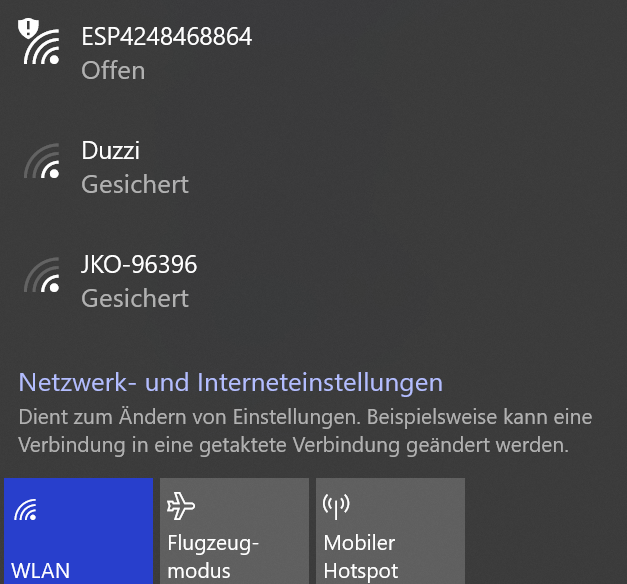
\includegraphics[width=0.5\textwidth]{graphics/WifiNetz.png}
	\caption{Esp Acces Point}
	\label{pic: wifiNetz}
\end{figure} 
Sobald "verbinden" mit diesem Netzwerk gewählt wird, startet der Browser eine Konfigurationsseite mit der IP Adresse des Targets. Nun ist ein Menü ersichtlich mit folgenden Wahlmöglichkeiten, siehe Abbildung \ref{pic: wifiNetz}:

\begin{figure}[H]
	\centering
	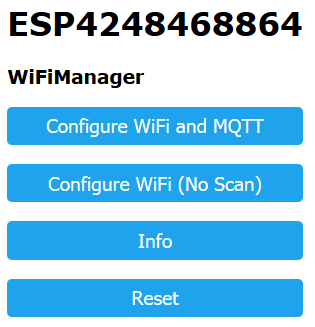
\includegraphics[width=0.5\textwidth]{graphics/WifiHome.png}
	\caption{Esp Konfiguration Home Menu}
	\label{pic: wifiHome}
\end{figure}   

Wird 'Configure WiFi and MQTT' angewählt erscheint folgende Ansicht in Abbildung \ref{pic: wifiKonfig}.

\begin{figure}[H]
	\centering
	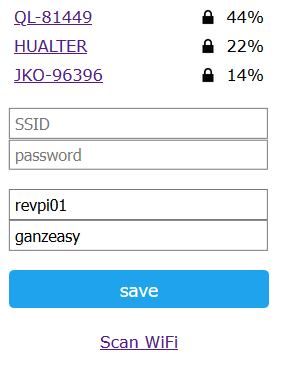
\includegraphics[width=0.5\textwidth]{graphics/WifiKonfig.png}
	\caption{Esp Konfiguration WiFi und MQTT}
	\label{pic: wifiKonfig}
\end{figure}   

Netzwerke, welche in der Umgebung gefunden wurden, werden angezeigt, die Parameter die zur WiFi Verbindung notwendig sind, können nun eingegeben werden. Im unteren Teil wird eine Voreinstellung der MQTT-Brocker-Adresse angezeigt und dessen Passwort, diese können beliebig geändert werden. Im WiFiManager Hauptmenü können die gleichen Konfigurationen ohne, dass nach vorhandenen Netzen gesucht wird, mit dem 'Configure WiFi(No Scan)' Button, gemacht werden. Mit dem Info Button werden Folgende Informationen angezeigt ChipID, Soft AP IP und Soft AP MAC wie auch Station AP MAC Adresse.

\begin{figure}[H]
	\centering
	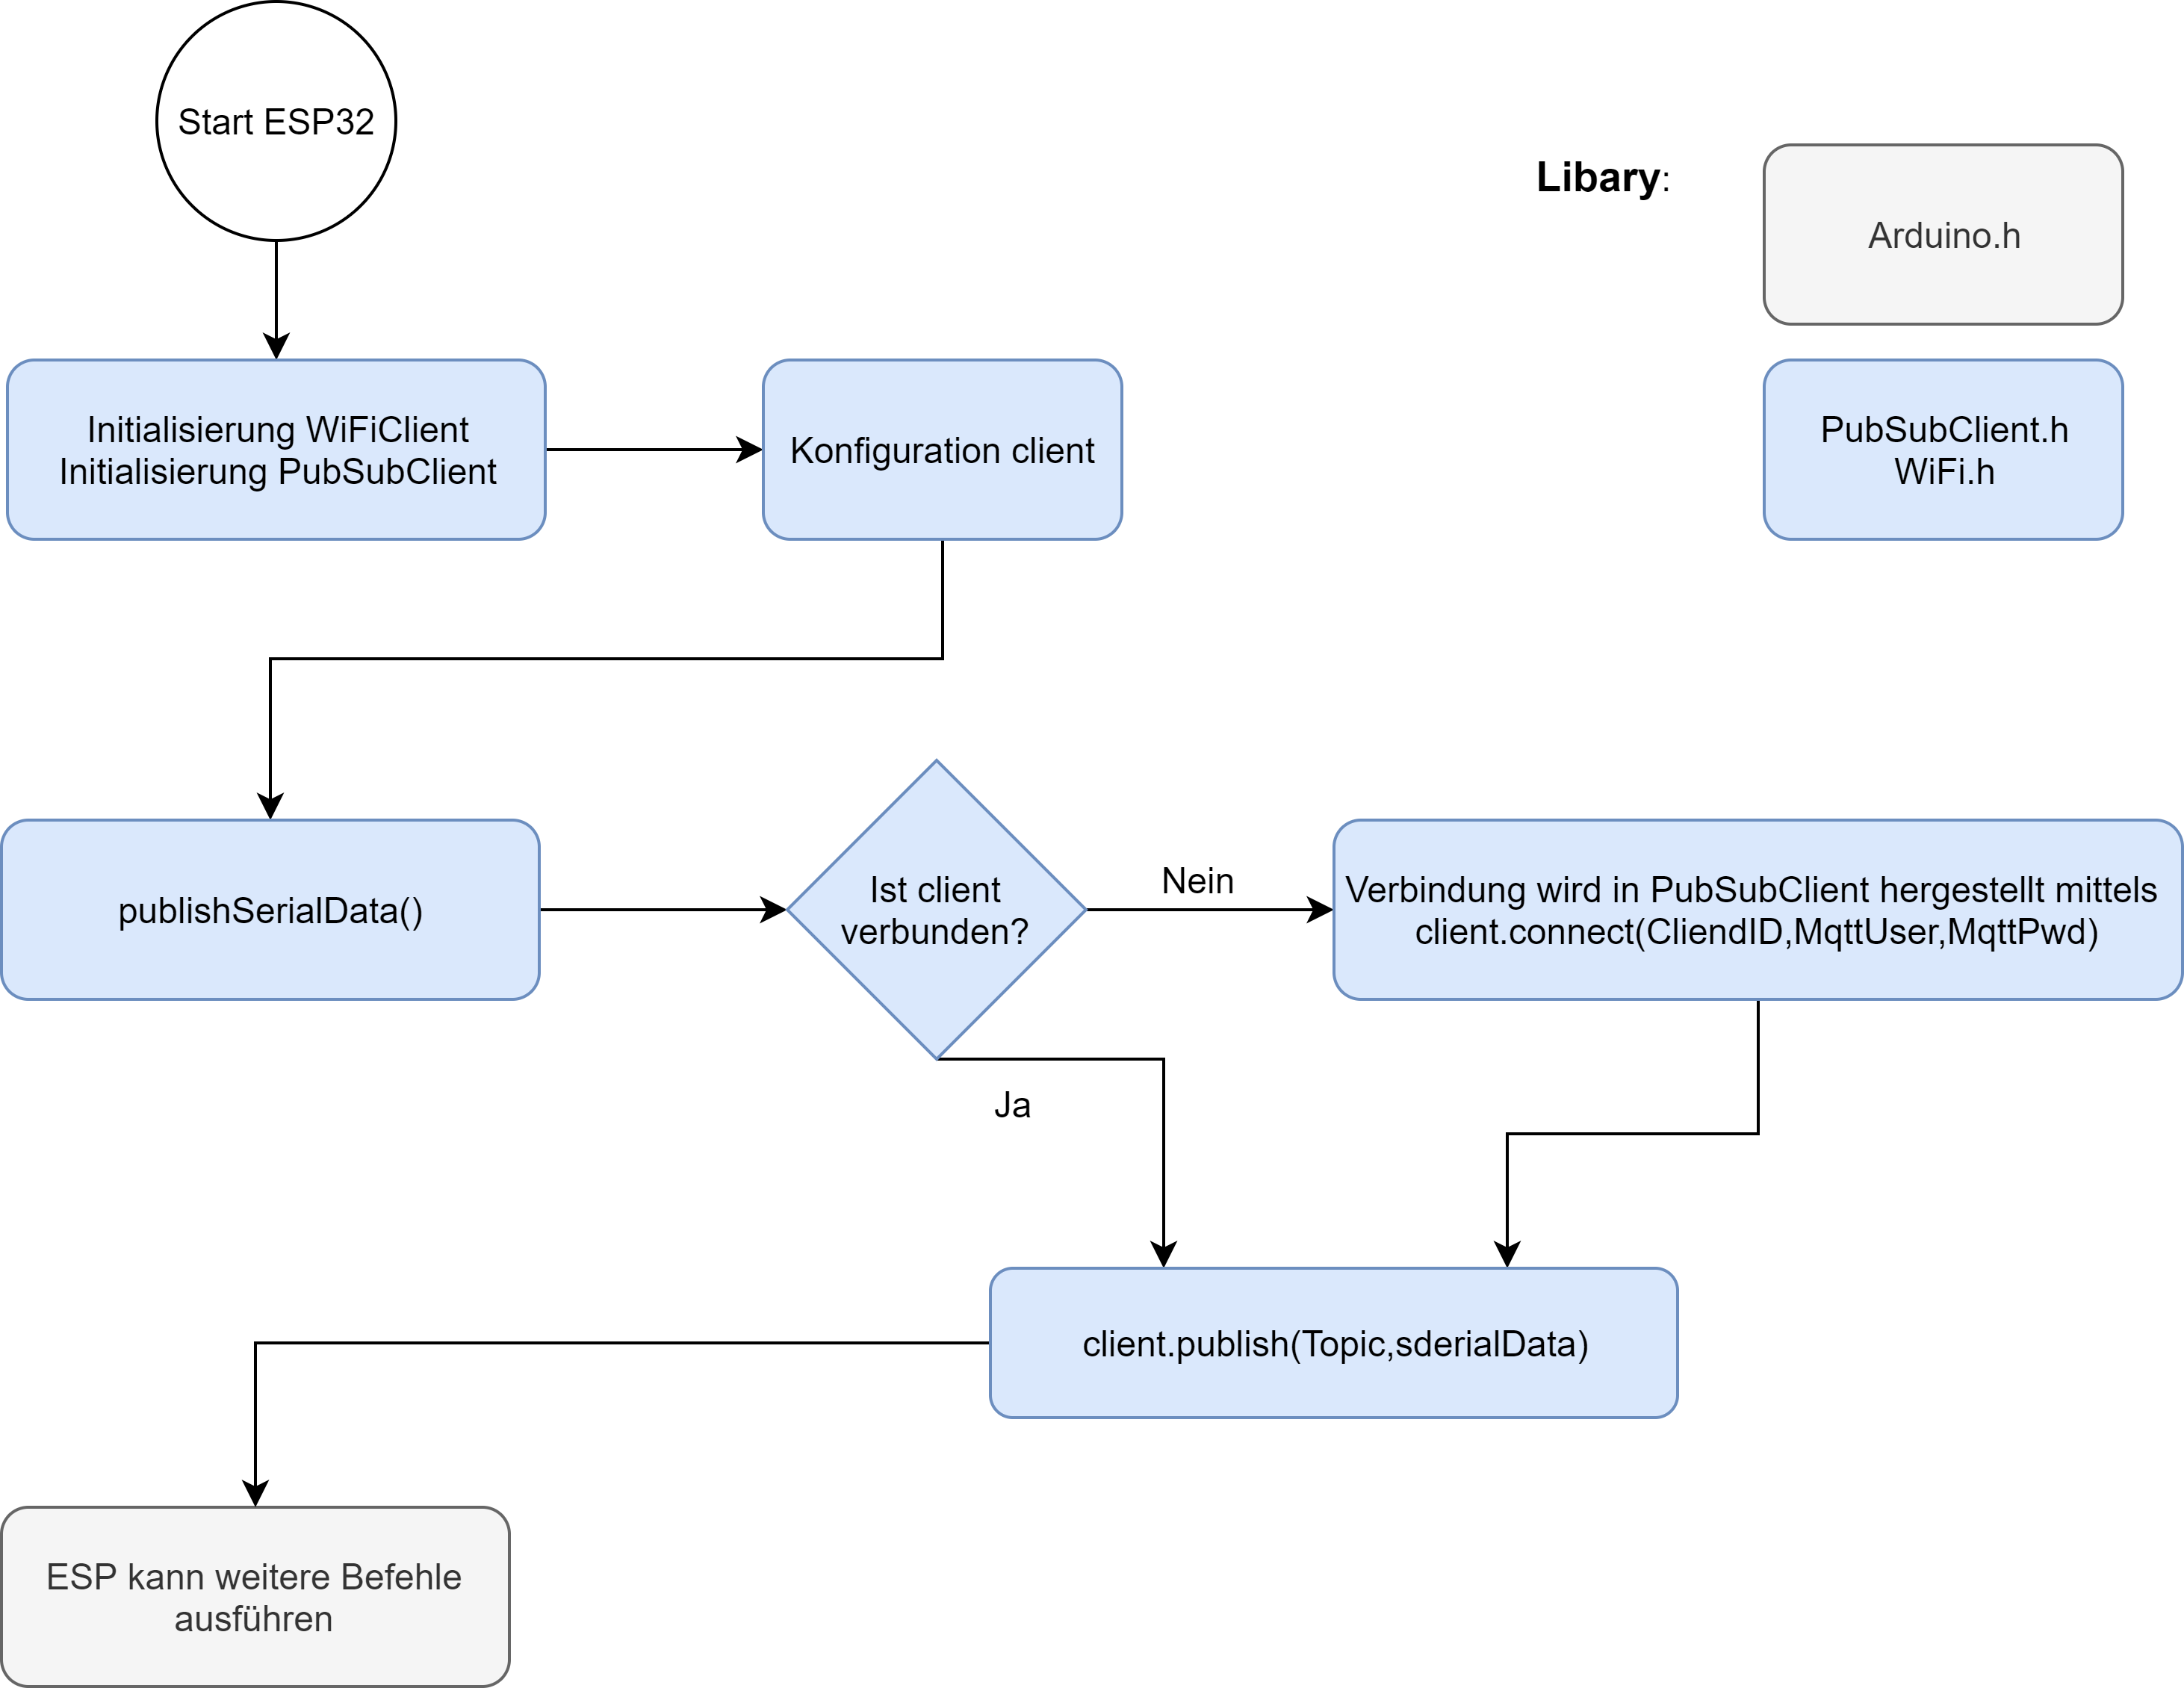
\includegraphics[width=\textwidth]{graphics/MQTTSubPubClient.png}
	\caption{Esp Info}
	\label{pic: SubPubClient}
\end{figure}   

Die für die MQTT-Kommunikation wird die Libary PubSubClient.h eingebunden. Als erstes wird der WiFiClient initialisiert. 

Danach wird der PubSubClinet als Client instantiiert, für diesen Vorgang werden folgende Parameter benötigt:\\
\begin{itemize}
\item 	server: Adresse von MQTT-Server\\
\item 	port: der Port von dem MQTT-Server\\
\item 	client: eine Instanz vom Ethernet-Client.\\
\end{itemize}
Die Funktion publishSerialData() ermöglicht, eine Nachricht zu veröffentlichen, bei diesem Vorgang wird den Topic und die seriellen Daten veröffentlicht. Beim Aufruf dieser Funktion, wird jedes mal überprüft ob die Verbindung zum MQTT-Borcker in Ordnung ist. 

Ist die Verbindung nicht in Ordnung, wird sie mit der Funktion connect(), hergestellt. Um diesen Prozess erfolgreich durch zu führen werden, CliendID, MQTT-Benutzername und Passwort benötigt.

Ist die Verbindung in Ordnung werden die Daten mit dem Befehl publish() veröffentlicht \cite{noauthor_arduino_nodate-1}.

\subsection{Programmcode Sensorbord}
Die Aufgabe welcher der Mikrocontroller vom Sensorboard  übernehmen besteht darin, dass er Betätigungen der Touchtasten auf dem Frontprint erkennt. Jeder Touchtaster besitzt ein LED mit dem das Betätigen bestätigt wird. Diese Funktion wurde so initialisiert, damit der User eine sofortige Kenntnis über die ausgelöste Aktion bekommt. Mit dem Sensorboard wird auf dem Frontprint die Umgebungstemperatur gemessen.



\subsubsection{	Übersicht} 
\begin{figure}[H]
	\centering
	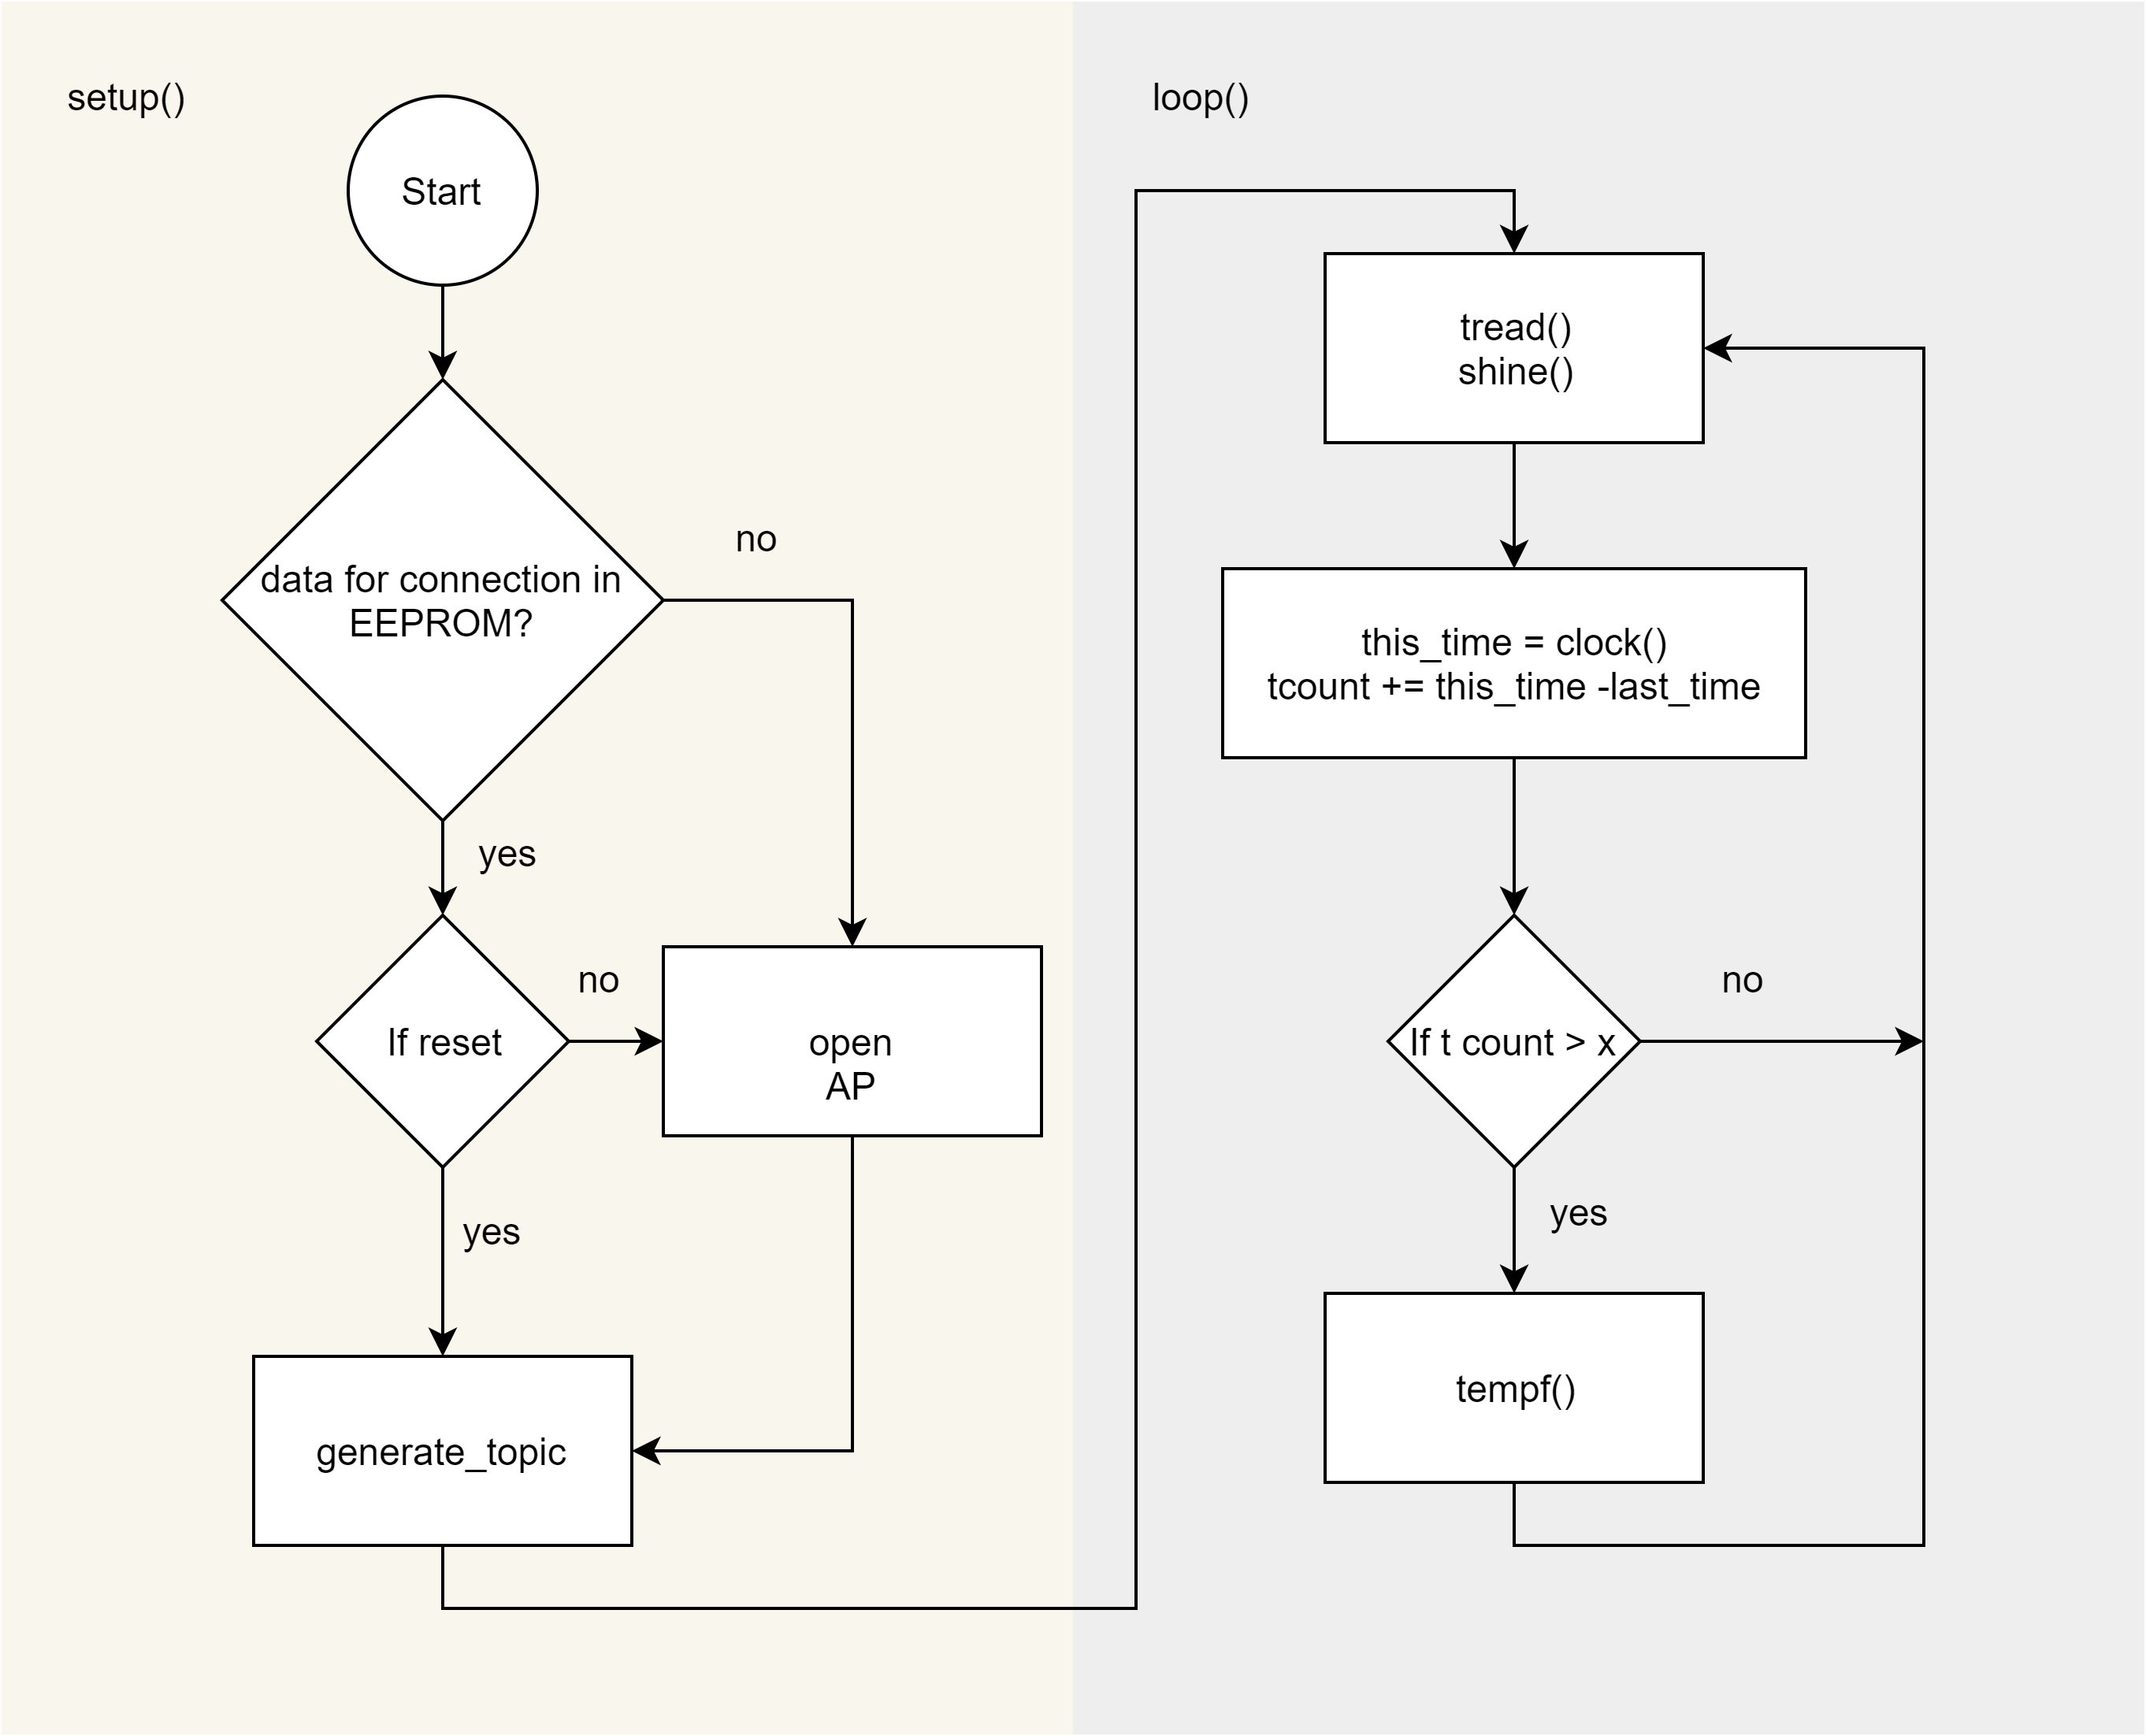
\includegraphics[width=\textwidth]{graphics/StatemaschineSensor.png}
	\caption{In dieser Abbildung ist das Statediagram vom Sensorboard abgebildet}
	\label{pic: statemaschine sensor}
\end{figure} 

\subsubsection{setup()}
Wird der Mikrocontroller gestartet so werden als erstes Configurations-Daten im EEPROM gesucht. Werden keine Daten gefunden oder wird die Reset-taste betätigt wird ein Accespoint eröffnet und Confugurations Parameter können mittels Browser eingegeben werden. Dieser Vorgang wird im Kapitel Kommunikation genauer beschrieben. Als nächster Schritt werden für die MQTT-Messages die Topics anhand der Bordbezeichnung und der Anwendung generiert. Die Bordbezeichnung wird im Configportal eingegeben und im EEPROM abgespeichert, sie dient dazu, wenn mehrere Boards installiert werden um die empfangenen Nachrichten zu unterscheiden. Eine mögliche Topic für eine MQTT Nachricht wenn beispielsweise der erste Taster betätigt wird kann folgendermassen aussehen: "data/sesnorboard/wohnzimmer/S1" in diesem Fall wurde die Bordbezeichnung Wohnzimmer gewählt. 

\subsubsection{loop()}
Im loop() wird als erstes die Funktion tread(), dann shine() aufgerufen, danach wird die Momentane Zeit mit der Funktion clock() geholt. In der Variabel count wird die Zeitdifferenz zwischen den wiederholenden Durchgängen von touch() addiert. Dies passiert solange bis der Wert x erreicht ist, in diesem Fall alle 10 Sekunden. Wenn der Wert x erreicht ist wird die Funktion tempf() aufgerufen, mit dieser wird mittels NTC die Temperatur gemessen. Im gleichen Zyklus wie die Temperaturmessungen Durchgeführt werden, wird die Staus LED geschaltet, so kann überprüft werden, ob sich das Bord im normalen Betrieb befindet, sprich der loop() wird gewiss komplett Durchlaufen. Die Funktionen sind in der nachfolgenden Abbildung abgebildet und werden anschliessend erläutert.

\begin{figure}[H]
	\centering
	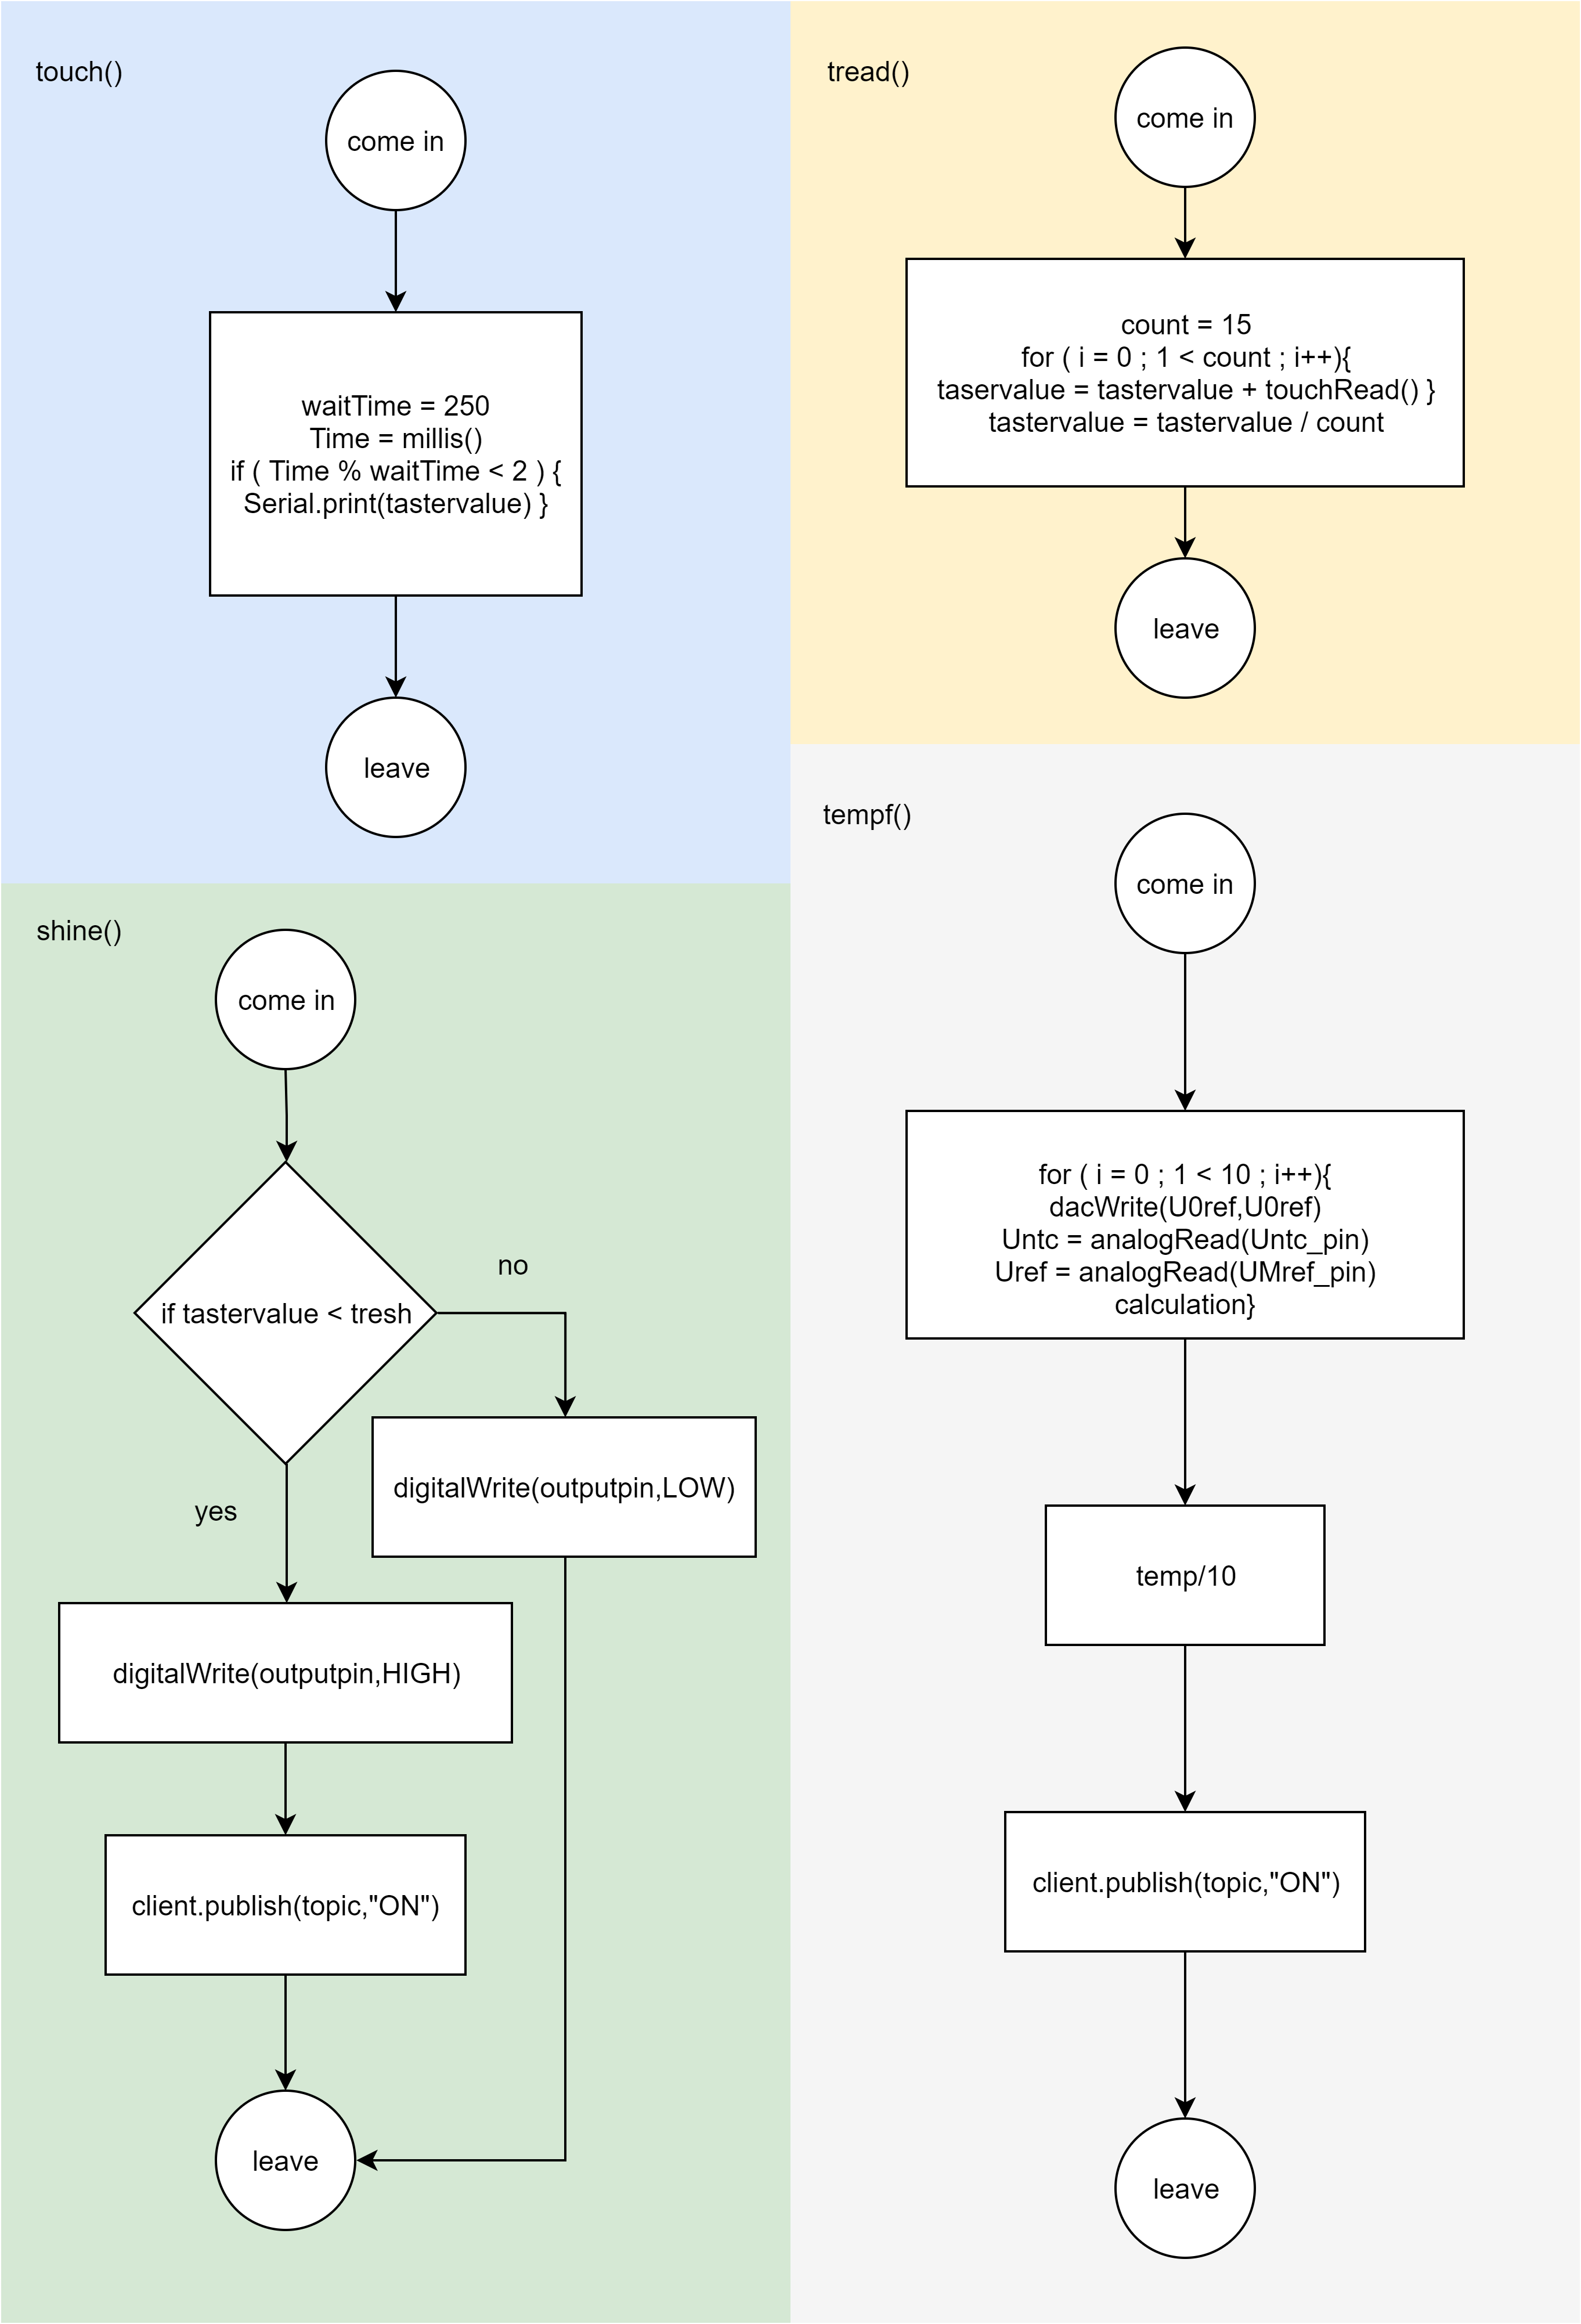
\includegraphics[width=\textwidth]{graphics/FunktionenSensor.png}
	\caption{In dieser Abbildung sind die Funktionen vom Sensorboard abgebildet}
	\label{pic: funktionen sensor}
\end{figure}   
\subsubsection{touch()}
Wie in der Abbildung \ref{pic: statemaschine sensor} zu erkennen ist, wird die Funktion touch() nicht aufgerufen. Sie dient alleine zum debuggen also um den optimalen tresh Wert zu finden. Dieser Wert definiert ab wann die Touchsensoren als gedrückt erkannt werden. In der Funktion wird die Variabel waitTime initialisiert mit dem wert 250 weiter wird der Wert millis() in die Variable Time gesetzt. In einer for-wihle werden so lange Time modulo waitTime kleiner als 2 sind, sprich die ersten 2 Millisekunden von 250 Millisekunden, mit Serial.prinln() der aktuell eingelesene Touchwert ausgegeben. Dieser Wert befindet sich im Ruhezustand um 50-80, wenn eine entsprechende Touch-Taste betätigt wird sinkt dieser Wert auf 10-30.  
\subsubsection{shine()}
In der Funktion shine() wird in einer for-while der Eingelesene Wert das sogenannte taservalue der jeweiligen Touchtasten mit dem Tresholdwert, tresh verglichen. Ist das tastervalue kleiner als tresh, wird eine MQTT-Message mit der entsprechenden Topic und der Payloud "ON" published. Ebenso wird die Led der entsprechenden Taste HIGH gesetzt. Trifft der andere Fall zu, wenn das tastervalue grösser als tresh ist wird die entsprechende Led LOW gesetzt.
\subsubsection{tread()}
In der Funktion tread() werden in einer for-while die aktuellen Werte der vier Touch-Tasten eingelesen und in den int-array tastervalue gesetzt, um Ausreisser zu eliminieren, wird ein Mittelwert erstellt. Es werden jeweils 15 Messungen addiert und aschliessend durch die Anzahl Messungen dividiert.  
\subsubsection{tempf()}
In dieser Funktion wird die Temperatur mit dem NTC ermittelt. In einer for-wihle wird der Analogwert am NTC in die Variabel Untc gesetzt ebenso wird der gemessene Referenzwert am Spannungsteiler gemessen. Nach der Umwandlung vom eingelesenen Wert des ADCs in Volts mit der Formel \todo{referenz formel adc}, wird anschliessend der Wert des Widerstands aus dem Spannungsteiler berechnet \todo{(ref auf Formel)}. Der Wert des Widerstand wird mit der Formel \todo{formel} in Grad $°C$ umgerechnet. Der gesamte Vorgang wird 10 mal wiederholt, damit der Mittelwert ermittelt werden kann. Der berechnete Temperaturwert wird von float in ein char umgewandelt und mit MQTT published. 
\newpage
\subsection{Programmcode Aktorbord}
Die Aufgabe des Aktorbord besteht darin, dass Befehle empfangen, verarbeitet und ausgeführt werden. Es befinden sich vier Relais auf dem Bord,welche 230 Volt schalten können, diese werden mit Digitalen IO Pins angesteuert. Eine weitere Aufgabe ist die Ausgabe von zwei DC-Spannnugen 0-10.  


\subsubsection{	Übersicht} 
\begin{figure}[H]
	\centering
	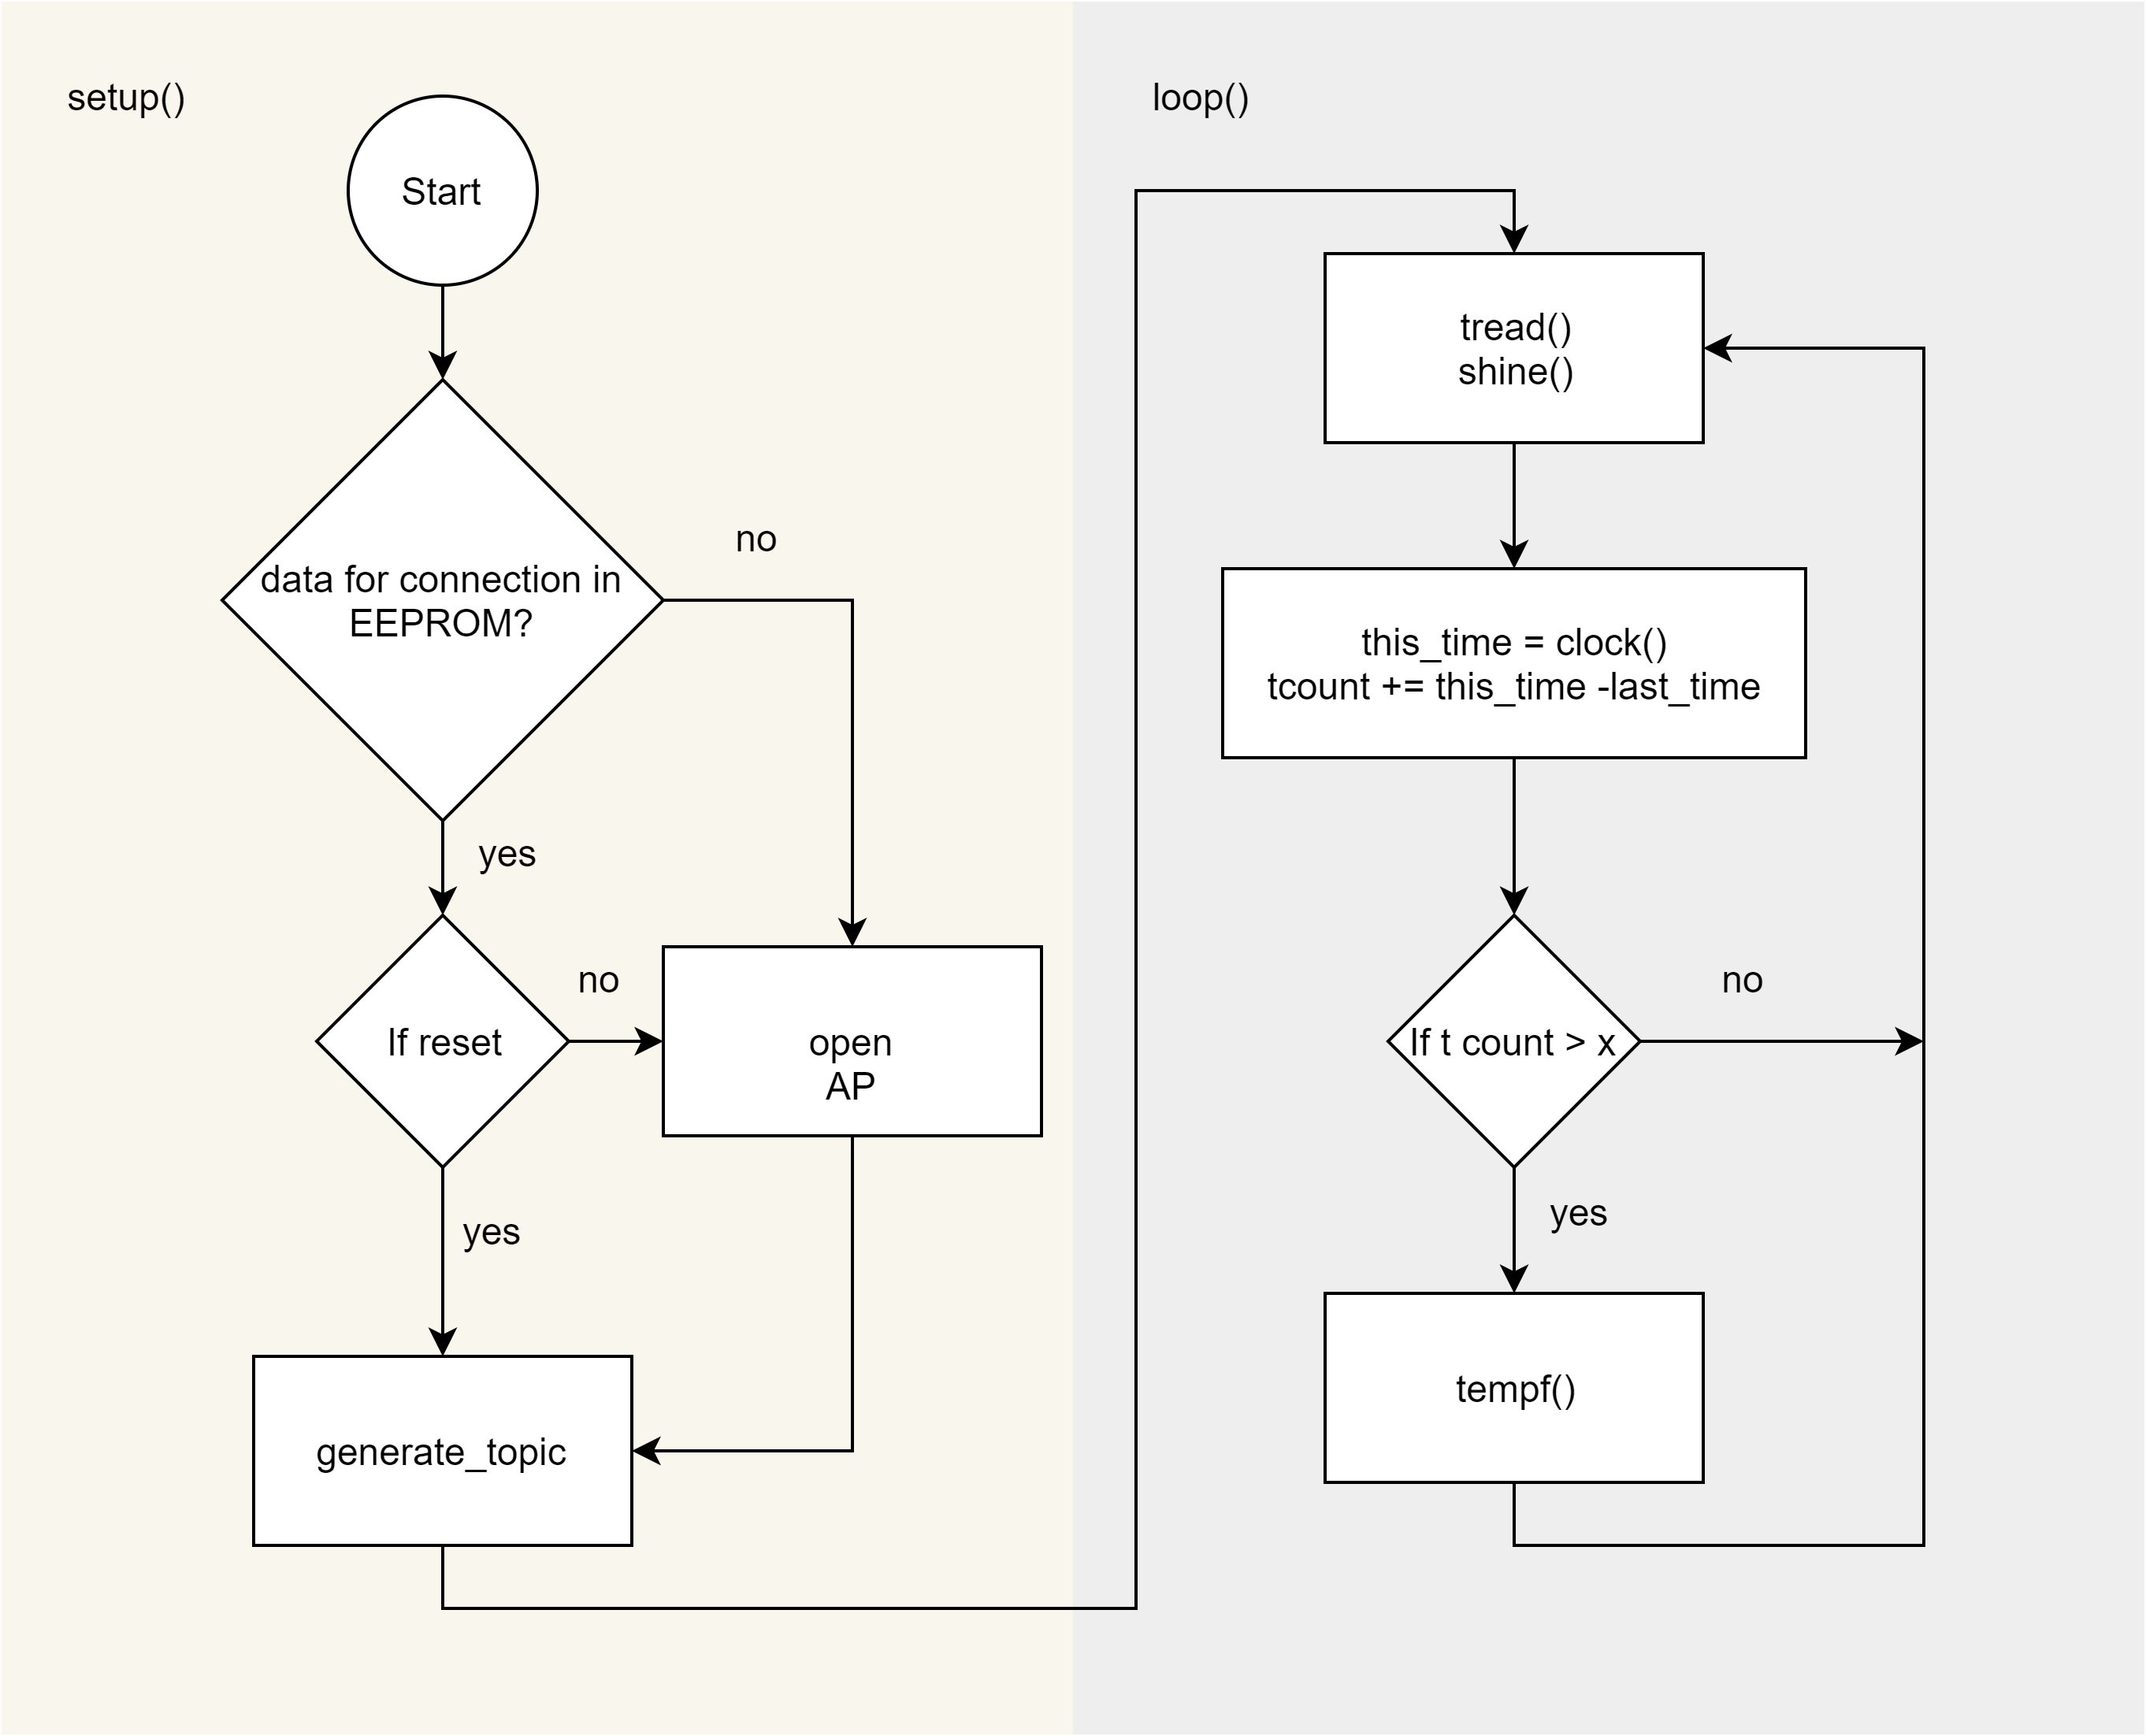
\includegraphics[width=0.5\textwidth]{graphics/StatemaschineSensor.png}
	\caption{In dieser Abbildung ist das Statediagram vom Sensorboard abgebildet}
	\label{pic: statemaschine sensor}
\end{figure} 
   
\subsubsection{Lizenzen} \todo{anpassen auf github min 1 ganze Seite, veröffentlichen usw}
Die Bibliotheken welche in den Kapiteln \ref{subsub: Wlan Konfiguration} , \ref{subsec: Framework} erwähnt wurden, sind freie Softwarepakete und können unter der Bedingung der GNU Lesser General Public Lizenz (LGPL) geändert werden. Die LGPL gibt die Freiheit das Programm, für jeden Zweck auszuführen, anzupassen und die Änderungen zu veröffentlichen. \cite{noauthor_gnu.org_nodate}.


 
